\documentclass[11pt]{beamer}
\usetheme{Montpellier}
\usepackage[utf8]{inputenc}
\usepackage[francais]{babel}
\usepackage{amsmath}
\usefonttheme{professionalfonts}
%\usepackage{fontspec}
\usepackage[T1]{fontenc}
%\setsansfont{Bitstream Charter}
%\setmainfont{Bitstream Charter}
%\defaultfontfeatures{Ligatures=TeX}
%\usepackage{unicode-math}
%\setmathfont{Tex Gyre Pagella Math}
%\setsansfont{Consolas}
%\fontspec{Lobster Two}
\usepackage{amsfonts}
\usepackage{amssymb}
\usepackage{graphicx}
\author{Ludovic}
\title{Une présentation Beamer de plus}
\setbeamercovered{transparent} 
%\setbeamertemplate{navigation symbols}{} 
%\logo{} 
\institute{Université de Savoie Mont Blanc} 
\date{01/01/2000} 
%\subject{} 
\begin{document}

\begin{frame}[plain]
\titlepage
\end{frame}

\begin{frame}
\tableofcontents
\end{frame}

\section{Introduction}
\subsection{Remarques introductives}

\begin{frame}{On commence ici}
  \begin{block}{Des choses importantes}
    \begin{itemize}
      \item Une choses,
      \item Une autre chose.
    \end{itemize}
  \end{block}
\end{frame}

\begin{frame}{Un autre transparent}
  \begin{columns}[c]
    \begin{column}{.6\textwidth}
      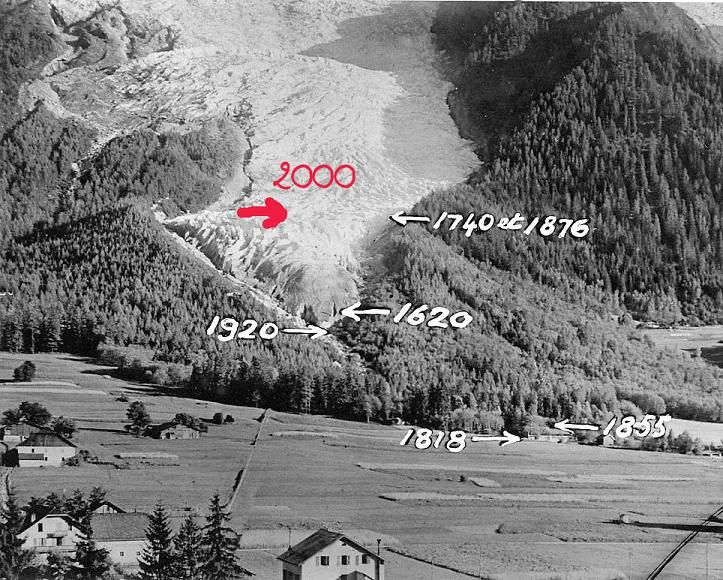
\includegraphics[width=\textwidth]{bossons}
    \end{column}
    \begin{column}{.4\textwidth}
      \begin{block}{Le glacier des Bossons}
        \begin{enumerate}
        \item<1,3> C'est de la glace,
        \item<2-> Il fond,
        \item<3> Il est blanc. 
        \item<4>
        \item<5>       
        \end{enumerate}
      \begin{equation}
      2 + 2 = \uncover<2>{3}
      \end{equation}        
      
      \end{block}         
    \end{column}
  \end{columns}
\end{frame}

\begin{frame}{La parabole}
\begin{columns}[c]
    \begin{column}{.6\textwidth}
      \includegraphics<1>[width=\textwidth]{parabola_1}
      \includegraphics<2>[width=\textwidth]{parabola_2}
    \end{column}
\begin{column}{.5\textwidth}
      \begin{block}{Le glacier des Bossons}
        \begin{enumerate}
        \item<1-> Une parabole,
        \item<2> Deux racines réelles.
        \end{enumerate}
      
      \end{block}         
    \end{column}
  \end{columns}

\end{frame}

\end{document}